% !TEX root = deplump.tex
\section{Algorithm}
\newcommand{\T}{\ensuremath{\mathcal{T}}}
\newcommand{\N}{\ensuremath{\mathcal{N}}}
\newcommand{\M}{\ensuremath{\mathcal{M}}}
\newcommand{\PP}{\ensuremath{\mathcal{P}}}
\newcommand{\nc}{\ensuremath{nc}}
\newcommand{\RS}{\ensuremath{\mathcal{R}}}
\newcommand{\D}{\ensuremath{\mathcal{D}}}
\newcommand{\la}{\ensuremath{\leftarrow}}
\newcommand{\G}{\ensuremath{\mathcal{G}}}
\newcommand{\IS}{\ensuremath{\mathcal{I}}}
\newcommand{\Seq}{\ensuremath{\mathcal{S}}}
\newcommand{\dd}{\ensuremath{\delta}}
%
%\begin{figure*}[t] 
%	\begin{center}
%		\scalebox{.6}{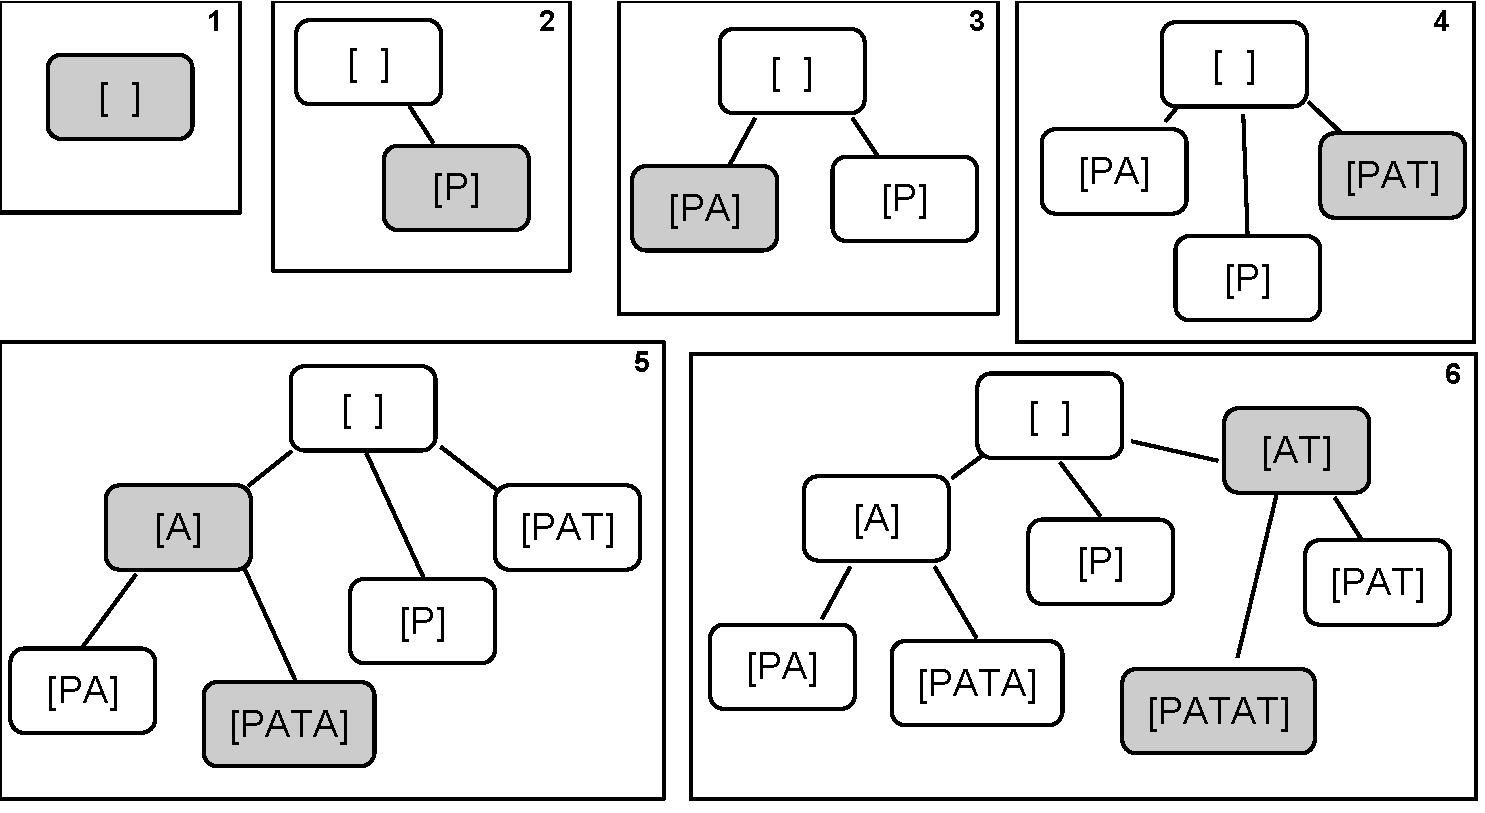
\includegraphics{figs/PATAT.pdf}} % [clip=true, viewport= 1in 1in 9in 9in]
%		\caption{Construction of suffix tree for string ``PATAT".  In each frame the new nodes are shaded in gray.}
%		\label{fig:suffix_tree}
%	\end{center} 
%\end{figure*} 
%
\begin{algorithm}[t!]
    \caption{Deplump/Plump} \label{alg:deplump/plump}
    \begin{algorithmic}[1]
    	\Procedure{$\mathcal{O}\mathcal{S} \la $ Deplump/Plump}{$\IS$}
		\State $\RS \la [$ $]$ ;  $\mathcal{O}\mathcal{S} \la  [$ $]$%\Comment{reference sequence}
%		\State Initialize $[$ $]$ node of \T \Comment{suffix tree}
		\State $\nc \la 1$ \Comment{node count}
		\State $\D \la  \{ \dd_0, \dd_1, \dd_2, \dots, \dd_{10}, \alpha \}$ \Comment{discount parameters}
% \Comment{output sequence}
		\For{i = 1: $| \IS|$}
			\State $\G \la \vec 0$ \Comment{discount parameter gradients, $|\G| = |\D|$}
			\State $ \{ \pi, \N  \} \la$  \textsc{PMFNext} (\RS)
			\If{Plump}
%				\State $s \la $ 
				\State $\mathcal{O}\mathcal{S} \la [\mathcal{O}\mathcal{S}$,  \textsc{RangeDecode}$(\pi, \IS)]$
			\Else
				\State $s \la \IS[i]$
%				\State $b \la$
				\State $\mathcal{O}\mathcal{S} \la [\mathcal{O}\mathcal{S}$,   \textsc{RangeEncode}$(\Sigma_{i = 1}^{s-1} \pi_i, \Sigma_{i = 1}^{s} \pi_i)]$		
			\EndIf
			\State \textsc{UpdateCountsAndDiscountGradients}($\N,s,\pi_s,$TRUE)
			\State $\D \la \D + \G \eta / \pi_s$ \Comment{update discount parameters}
			\State $\RS \la [\RS$ $s]$ \Comment{append symbol to reference sequence}
		\EndFor
%		\State \Return $\mathcal{O}\mathcal{S}$
	\EndProcedure
	\end{algorithmic}
\end{algorithm}

Our focus in this section is on providing the first comprehensive implementation reference for deplump with the changes necessary to achieve streaming asymptotics highlighted.  Many of the individual algorithms that appear in this section are justified and explained in detail in prior art.  We explain the functionality of each algorithm, but refer the interested reader to the prior art for detailed mathematical justifications, in particular \citep{Wood2009,Gasthaus2010,Bartlett2010}.

Given a sequence of symbols $\Seq = [s_0, s_1, s_2, \ldots]$ where each symbol $s_n$ comes from from an ordered set of symbols $\{\sigma_0, \sigma_1, \ldots\} = \Sigma$,  streaming deplump works by repeatedly producing a predictive distribution for the continuation of the sequence given the full preceding context and encoding the next symbol by passing that predictive distribution to an entropy encoder.  In this paper explicit details related to encoding and decoding are not included, instead we present the algorithms necessary to incrementally construct the predictive distributions needed by the encoder and decoder.  Specifically, we assume that if the predictive distribution function is $F$ and the next symbol in the stream is $s$ then the stream can be compressed using an entropy encoder that takes $F(s-1)$ and $F(s)$ as arguments and returns a bit stream (possibly null) \citep{Witten1987}.   The cumulative distribution function is well defined because the symbols are ordered. We use the notation $s-1$ to refer to the symbol prior to $s$ in the symbol set $\Sigma$.  %Note that the symbol set can be ordered as the set is discovered.
%Further, although there is a beautiful interplay between the algorithms presented herein and approximate inference in the underlying model, we have decided to, given the availability of referenced work on 
\begin{figure*}[ttt!]
	\begin{minipage}[t]{.48\linewidth}
		\begin{algorithm}[H]
			\caption{PMFNext} \label{alg:pmfnextsymbol}
	\begin{algorithmic}[1]
	\Function{$\{ \pi, \N \} \la $ PMFNext}{$\RS$}
		\While{$ |\RS| \geq T$}
%			\State Delete nodes referencing \RS[1] and update $nc$
			\State $\RS \la \sigma(\RS)$
		\EndWhile
		\While{ $\nc > (L - 2)$}
			\State Delete random leaf node
			\State $nc \la nc -1$
		\EndWhile
		
		\State $\N \la$ \textsc{GetNode}$(\RS, \T)$
		\State $\pi \la$ \textsc{PMF}($\N, \vec 0, 1.0$) \Comment{$| \vec 0| = | \Sigma|$}
	%	\State UpdateCountsAndDiscountGradients($\N,s,\pi_s,$TRUE)
%		\State \Return [$\pi$, \N]
	\EndFunction
	 \end{algorithmic}
\end{algorithm}
\vspace{-.75cm}
\begin{algorithm}[H]
	\caption{DrawCRP} \label{alg:drawcrp}
	\begin{algorithmic}[1]

	\Function{$t \la $ DrawCRP}{$n,d,c$} %\Comment{$ n \geq 1$}
		\State $t \la 1$
		\For{i = 2 : n}
			\State $r \la 0$
			\State $r  \la 1$ w.p. $\frac{td + c}{i-1 + c}$
			\State $t \la t + r$
		\EndFor
%		\State \Return $t$
	\EndFunction
	
	\end{algorithmic}	
\end{algorithm}
	 \end{minipage}
	\hfill
%
%
%%\begin{algorithm}
%	\caption{GetDiscount} \label{alg:getdiscount}
%    \begin{algorithmic}[1]
%    	\Function{PointOnCDFNextSymbol}{$h,\T,\RS$}
%		\While{$ |\RS| \geq 100 L$}
%			\State Delete nodes referencing \RS[0]
%			\State $\RS \la \sigma(\RS)$
%		\EndWhile
%		\While{ $\nc > (L - 2)$}
%			\State Delete leaf node uniformly at random
%		\EndWhile
%		\State $\N \la$ GetNode$(\RS, \T)$
%		\State $\pi \la$ PMF($\N, \vec 0, 1.0$) \Comment{$| \vec 0| = | \Sigma|$}
%		
%		\State $F(s) \la 0$
%		\State $s \la 0$
%		\While{$F(s) < h$}
%			\State $s \la s + 1$
%			\State $F(s) \la F(s) + \pi_s$
%		\EndWhile
%		
%		\State $F(s-1) \la F(s) - \pi_s$
%		\State Update $h$
%		\Return  $[h,s, F(s-1), F(s)]$
%	\EndFunction	
%	\Function{GetDiscount}{\N}
%		\State $d = 1.0$
%		\If{\N = [ ]}
%			\State \Return $\dd_0$
%		\EndIf
%		\For{$i = (|$\textsc{PA}$(\N)| + 1): |\N|$}
%			\If{$i \leq 10$}
%				\State $d \la d \delta_i$ \Comment{multiply by discount parameter $i$}
%			\Else
%				\State $d \la d \dd_{10}^{\alpha^i}$
%			\EndIf
%		\EndFor
%		\State \Return $d$
%	\EndFunction
%	
%		\end{algorithmic}
%\end{algorithm}
	\begin{minipage}[t]{.48\linewidth}
\begin{algorithm}[H]
	\caption{GetNode} \label{alg:getnode}
	\begin{algorithmic}[1]
    	\Function{$\Seq \la $ GetNode}{\Seq, \T}
		\State Find the node \M \space in the tree sharing the longest suffix with \Seq
		\If{\M \space is a suffix of \Seq}
%			\If{$\Seq = \M$ or $|\M| = D$}
%				\State \Return \M
			\If{$\Seq \neq \M$ and $|\M| <  D$}
				\State $\Seq \la$ \textsc{CreateNode}$(\Seq, \M)$
				\State $nc \la nc + 1$
%				\State \Return \Seq
			\EndIf
		\Else
			\State \PP \la \space \textsc{FragmentNode}(\M, \Seq)
			\State $\Seq \la $ \textsc{CreateNode}$(\Seq, \PP)$
			\State $nc \la nc + 1$
%			\State \Return \Seq
		\EndIf
	\EndFunction
	\end{algorithmic}	
\end{algorithm}
	\end{minipage}
	\end{figure*}

The algorithms of deplump run over a constant space, incrementally constructed suffix-tree-like data structure.  Note that the fact that this datastructure is of constant size is a significant point of  differentiation between this work and that of \cite{Gasthaus2010}. This tree-shaped data structure efficiently encodes a subset of the set of unique suffixes of all contexts in a sequence.  Each edge in the tree has a label which is a subsequence of the input sequence.  Each edge label is represented by two indices into a fixed-length suffix of the input sequence which we call the reference sequence (i.e.~each edge label is $[r_{i+1}, r_{i+2}, \ldots,r_{j}]$ for indices $i$ and $j$ into the reference sequence where $[r_{1} = s_{n-T}, \ldots, r_T = s_n]$ after every $n$th input sequence element is processed.)  
Therefore, each node in the tree corresponds to a subsequence $[s_m, \ldots, s_{m + k}]$ of the input sequence and a (potentially non-sequential) set of subsequences of the reference sequence.  
%The suffix a node corresponds to is determined by concatenating the edge labels on the path from the root to the node. (i.e.~the set $\{ [ ], [s_0], [s_0,s_1], [s_0, s_1,s_2], \ldots \}$)
We use $\N$ to refer interchangeably to a node and the suffix in the input sequence to which the node corresponds.  Note that for a given suffix the corresponding node is accessed by traversing edges of the tree that match the suffix read from right to left. 
\begin{algorithm}[t!]
	\caption{UpdateCountsAndDiscountGradients} \label{alg:updatecountsandgradients}
	\begin{algorithmic}[1]
	
	\Function{UpdateCountsAndDiscountGradients}{$\N, s, p$, BackOff}
	%	\State $d \la $ \textsc{GetDiscount}(\N)
		\State $pp \la p$
		\If{$c > 0$}
			\State $pp \la (p - \frac{c_s - t_s d^{\N}}{c}))(\frac{c}{t d^{\N}})$
			\State $w \la c_s	+ d^{\N}(t *pp - t_s)$		
		\EndIf
		
		\If{BackOff  and $c > 0$}
			\State $c_s \la c_s + 1$
			\State BackOff $\la 0$
			\State BackOff $\la 1$ w.p. $pp (\frac{t d^{\N}}{w})$ \Comment{w.p abbreviates ``with probability"}
			\If{BackOff}
				\State $t_s \la t_s + 1$
			 \EndIf
		\ElsIf{BackOff}
				\State $c_s \la c_s + 1$;  $t_s \la t_s + 1$
		\EndIf
		
		
		\State \textsc{UpdateDiscountParameterGradients}($t_s, t,pp, d^{\N}$)
		\State \textsc{UpdateCountsAndDiscountGradients}(\textsc{PA}(\N), $s,pp$, BackOff)
		\State \textsc{ThinCounts}(\N)
	\EndFunction
		\end{algorithmic}
\end{algorithm}

Streaming deplump is given in Algorithm~\ref{alg:deplump/plump}.  Deplump processes each element of an input sequence $\IS$ incrementally.  For each element $s_n$ of $\IS$, \textsc{PMFNext} computes the predictive probability mass function $\pi$ (conditioned on the observed context $[s_0, s_1, \ldots, s_{n-1}] = \RS$) needed for compression.  The element $s_n$ is then encoded by an entropy encoder with parameter $\pi$.  \textsc{PMFNext} also handles the incremental maintenance of the underlying constant-space datastructures by restricting the length of the reference sequence and by both constructing and deleting nodes in the tree as needed.  The final steps in streaming deplump are to incrementally integrate the observation into the approximated sequence memoizer and to adjust the back-off/smoothing parameters $\D$.  This involves updating counts in the tree and calculating a stochastic gradient for $\D$.  Both of these are done in \textsc{UpdateCountsAndDiscountGradients}. %The discount parameters are updated based on a learning rate $\eta$ and the encoded symbol in appended to $\RS$. 
The organization of functions in this way minimizes the number of tree traversals that need to be performed, tree traversals being a major component of the computational cost of this algorithm.

\textsc{PMFNext} (Alg.~\ref{alg:pmfnextsymbol}) starts by enforcing the bounds on $|\RS|$ and $|\mathcal{H}|$.  Both of these bounds require nodes to be removed from the tree (the first implicitly as a result of edge labels becoming undefined and the second explicitly).  Removing nodes from the underlying sequence datastructure has no consequence in and of itself, but as an operation on the corresponding sequence memoizer graphical model some care must be taken because node removal has ramifications in terms of what kinds of approximations are being imposed on inference.  \cite{Bartlett2010} showed that removing leaf nodes from the sequence memoizer results in a coherent approximate inference algorithm for the sequence memoizer.  So, enforcing the bound on $| \mathcal{H} | < L$ can be as simple as incrementally removing leaf nodes uniformly at random.  To facilitate random deletion we maintain a count in each node of the number of leaf nodes in the subtree below it.  A random leaf node can then be obtained by traversing a weighted random path down the tree.  

\begin{figure*}[ttt!]
\begin{minipage}[t]{.48\linewidth}
\begin{algorithm}[H]
	\caption{ThinCounts} \label{alg:thincounts}
	\begin{algorithmic}[1]
			
	\Function{ThinCounts}{$\N$}
	%	\State $d \la$ \textsc{GetDiscount}$(\N)$
		\While{$c > k$}
			\State $\pi = [\frac{c_{\sigma_1}}{c}, \frac{c_{\sigma_2}}{c}, \ldots, \frac{c_{\sigma_{|\Sigma}}}{c}]$
			\State $s \la $ \textsc{Multinomial}$(\pi)$ %s.t. $\pi_l = \frac{c_l}{c}$ % \Comment{$\pi$ is a distribution over $\Sigma$}
			\State $\phi \la$ \textsc{Partition}$(c_s, t_s, d^{\N})$
			\State $\psi \la (\frac{1}{c_{s}} ) \phi$
			\State $i \la$ \textsc{Multinomial}$(\psi)$
			\If{$\phi_i == 1$}
				\State $t_s \la t_s - 1$
			\EndIf
			\State $c_s \la c_s - 1$
		\EndWhile
	\EndFunction	
	
	\end{algorithmic}	
\end{algorithm}
\end{minipage}
\hfill
\begin{minipage}[t]{.48\linewidth}
\begin{algorithm}[H]
	\caption{PMF} \label{alg:pmf}
	\begin{algorithmic}[1]

	\Function{$\pi \la $ PMF}{$\N, \pi, m$}
%		\State $d \la $ \textsc{GetDiscount}(\N)		
		\If{$c > 0$}
			\For{$\sigma \in \Sigma$}
				\State $\pi_\sigma\la \pi_\sigma + m(\frac{c_\sigma - t_\sigma d^{\N}}{c})$
			\EndFor
		\EndIf
		
		\If{\textsc{PA}$(\N) \neq$ null}
			\State $\pi \la $ \textsc{PMF}(\textsc{PA}(\N), $\pi, d^{\N} m$)
		\Else
			\State $\pi \la (1- d^{\N} m)\pi + d^{\N}m\mathcal{U}_{\Sigma}$ %\Comment{$\mathcal{U}(\Sigma)$ is the uniform distribution over $\Sigma$}
%			\State \Return $\pi$
		\EndIf 
	\EndFunction
		\end{algorithmic}
\end{algorithm}
\end{minipage}
\end{figure*}

The removal of nodes due to their edge labels becoming undefined is an unfortunate consequence of having to constrain the reference sequence $\RS$ to be of constant length.  Note that without a bound $|\RS|$ would grow in length by one as each symbol of the input sequence is incorporated into the model.  To maintain the upper bound on $|\RS|$ we shorten $\RS$ by one as in a fixed length FIFO queue. Since the labels of edges in the tree index into $\RS$ then, when it is shortened, some edges may end up having labels that index beyond the retained elements of $\RS$ resulting in ``undefined'' edges.  Nodes below any undefined edges in the tree must be removed because they can no longer be accessed.  Their removal is justified in the same way as before because all subtree removals can be implemented as a cascade of leaf node removals.  It is desirable to minimize the number of nodes removed due to the incessant shortening of $\RS$.  One way to do this is to always update all edge indices on all paths traversed in the process of inserting nodes into the tree (that we do this is not made explicit in Alg.~\ref{alg:getnode} but on line 2 this updating of the edge indices should be performed)   \textsc{PMFNext} finishes by accessing the correct node for prediction using \textsc{GetNode} (Alg.~\ref{alg:getnode}) and the predictive probability mass function is calculated recursively by \textsc{PMF} (Alg.~\ref{alg:pmf}).

\begin{algorithm}[t!]
	\caption{FragmentNode} \label{alg:fragmentnode}
	\begin{algorithmic}[1]

	
	\Function{$\PP \la $ FragmentNode}{$\M, \Seq$}
%		\State $d^\M \la$ \textsc{GetDiscount}(\M)
		\State $\PP \la$ maximum overlapping suffix  of \M \space and \Seq
		\State $\PP \la $ \textsc{CreateNode}$(\PP,$ \textsc{PA}$(\M))$
		\State $nc \la nc + 1$
		\State\textsc{ PA}(\M) $\la \PP$
%		\State $d^\PP \la$ \textsc{GetDiscount}(\PP)
		\For{$\sigma \in \Sigma$}
			\State $\phi \la$ \textsc{Partition} $(c^\M_\sigma, t^\M_\sigma,d^\M)$
			\State $t^\PP_\sigma \la t^\M_\sigma$;  $t^\M_\sigma \la 0$
			\For{$i= 1 : | \phi|$}
				\State $a \la$ \textsc{DrawCRP}$(\phi[i],d^\M / d^\PP,-d^\M)$
				\State $t_\sigma^\M \la t_\sigma^\M + a$
			\EndFor
			\State $c^\PP_\sigma \la t^\M_\sigma$
		\EndFor
%		\State \Return \PP
	\EndFunction
		\end{algorithmic}
\end{algorithm}

Incremental construction of the tree is handled by the function \textsc{GetNode} within \textsc{PMFNext} which creates two or fewer nodes in the tree for every call.  Within the function \textsc{GetNode}, nodes are created by \textsc{CreateNode} and \textsc{FragmentNode}. The function \textsc{CreateNode(\N,\M)} simply creates a node $\N$ with parent $\M$. \textsc{FragmentNode} (Alg.~\ref{alg:fragmentnode}) implements the fragmentation operation developed in \citep{Wood2009} required to ensure proper sequence memoizer inference in the case where an edge must be split and a node inserted, but does so in the constant space node representation given in \citep{Gasthaus2011}.  This new intervening node corresponds to a predictive context and the counts corresponding to a proper estimate of this predictive distribution must be inferred.   Practically this means that value must be assigned to all counts $t_s^\mathcal{P}, c_s^\mathcal{P}, t_s^\mathcal{M}, c_s^\mathcal{M}$ for $s\in\Sigma$.  \textsc{FragmentNode} uses two functions to do this: \textsc{Partition}$(c,t,d)$ (Alg.~\ref{alg:samplepartition}) and \textsc{DrawCRP}$(n,d,c)$ (Alg.~\ref{alg:drawcrp}).  The net effect of \textsc{FragmentNode} is to create a new branching node at the shared suffix of $\mathcal{M}$ and $\mathcal{S}.$   The mathematical explanation of these algorithms is given in \citep{Gasthaus2011}.  % together implement the node fragmentation algorithm for the constant space node representation of the sequence memoizer discussed in \citep{Gasthaus2011}.% (this samples a partition following the $\mathcal{E}\mathcal{S}_{c}(d,0)$\footnote{ The two parameter Ewen's $\mathcal{E}\mathcal{S}_{n}(d,c)$ distribution is a distribution over partitions of $n$ objects and plays a key role in inference in models using Pitman-Yor distributions \cite{Ewens_dist_ref}.} distribution conditioned on the length of the partition being $t$).\textsc{DrawCRP}$(n,d,c)$ returns the length of a random partition drawn from the $\mathcal{E}\mathcal{S}_{n}(d,c)$.  %and is called when none of the existing tree nodes are a suffix of the context \RS.  
%An illustration of the incremental construction of a suffix tree can be seen in Figure~\ref{fig:suffix_tree} for the toy sequence [PATAT].  We use \textsc{PA}(\N) to refer to the parent of $\N$ in the tree.  In frame 4 the function \textsc{GetNode} assigns [ ]  to $\M$ and then [PAT] to $\Seq$ with $\M = \textsc{PA}(\Seq)$. In Frame 5 \textsc{GetNode} assigns [PA] to $\M$, but then must assign [A] = \textsc{FragmentNode}(\M) to $\PP$ and \textsc{PA}$(\M)$ to \PP.  Node $\Seq$ is then created by \textsc{CreateNode}$($[PATA]$,\PP)$.   % In each frame the first step is to find $\M$, which can be achieved by descending an appropriate path of the suffix tree.  All of the nodes on the path to $\M$ and possibly $\M$ itself can have the indices into $\RS$ updated to point to a more recent section of the reference sequence. 

\begin{algorithm}[t!]
	\caption{Partition} \label{alg:samplepartition}
	\begin{algorithmic}[1]
	
	\Function{$\phi \la  $ Partition}{$c,t,d$}
		\State $M \la  t \times c$ matrix of zeros
		\State $M(t,c) \la 1.0$
		\For{$j = (c-1) : 1$}
			\For{$i = 1 : (t-1)$} 
				\State $M(i,j) \la M(i +1, j+1) + M(i,j+1)(j - id)$ 
			\EndFor
			\State $M(d,j) \la M(t,j+1)$
		\EndFor
		\State $\phi \la [1,0,0,\ldots, 0]$ \Comment{$|\phi| = t$}
		
%		\State $\phi \la \vec 0$ \Comment{$|\vec 0| = t$}
	%	\State $\phi[1] \la 1$;  $k \la 1$
		\For{j = 2 : c}
			\State $M(k,j) \la M(k,j)(j-1 -k d)$
			\State $r \la 0$
			\State $r \la 1 $ w.p. $\frac{M(k+1,j)}{M(k+1,j) + M(k,j)}$
			\If{r = 1}
				\State $k \la k + 1$
				\State $\phi[k]  \la 1$
			\Else
				\State $i \la$ \textsc{Multinomial}$([\frac{\phi[1] - d}{j-1 -kd}, \frac{\phi[2] - d}{j-1 -kd}, \ldots, \frac{\phi[k] - d}{j-1 -kd}])$
				\State $\phi[i] \la \phi[i] + 1$
			\EndIf
		\EndFor
%		\State \Return $\phi$
	\EndFunction
		\end{algorithmic}
\end{algorithm}

Finally \textsc{UpdateCountsAndDiscounts} (Alg.~\ref{alg:updatecountsandgradients}) integrates the observation into the underlying probability model, adjusting counts in potentially all nodes on the path from the context in which the observation was made to the root of the context tree.   \textsc{UpdateCountsAndDiscounts} also computes a partial stochastic gradient for the discount parameter of each node on this path (this gradient is used in \textsc{Deplump} to update $\mathcal{D}$).  The details of the discount computation performed in \textsc{UpdateDiscountParameterGradients} are too long to include but can be obtained from \cite{Gasthaus2010}.  \textsc{UpdateCountsAndDiscounts} also uses \textsc{ThinCounts} (Alg.~\ref{alg:thincounts}) to enforce the bound on the counts in each node required to ensure computational asymptotics appropriate for streaming compression. 


%Each node instance $\N$ contains two counts for each $\sigma \in \Sigma$, $c_\sigma$ and $t_\sigma$.  We use $c$ and $t$ to refer to the marginal counts $\sum_{\sigma \in \Sigma} c_\sigma$ and $\sum_{\sigma \in \Sigma} t_\sigma$.  Each node also has a discount associated with it which we refer to as $d^\N$ in the algorithms. If we define $\delta_{n} = \delta_{10}^{\alpha^{n - 10}}$ for $n \geq 10$ then $d^{\N} = \Pi_{i =|\textsc{PA}(\N)| + 1}^{|\N|} \delta_{i}$ if $\N$ is not the root and $\delta_{0}$ if $\N$ is the root.  Counts are updated and discount parameter gradients are calculated by Algorithm~\ref{alg:updatecountsandgradients}.  The new approximation discussed in Section~\ref{section:methodology} is implemented by \textsc{ThinCounts}.

%The reference sequence grows with the length of the input sequence and must be shortened as the algorithm progresses.  When $\RS$ is shortened, nodes in the suffix tree which reference removed sections are no longer usable and must be removed from the tree to prevent a memory leak.  To facilitate the removal process pointers are maintained from the elements of $\RS$ to the suffix tree nodes which reference them.  Without the use of pointers, deletion of the unusable nodes requires a search over the tree which is prohibitive for large trees. The cost of these operations can be amortized by shorting $\RS$ in chunks and keeping pointers from each chunk of $\RS$ instead of each element.  

%The reference sequence $\RS$ is implemented as a linked list. Therefore, instead of using a simple $i,j$ index in each suffix tree node, $i$ is replaced by a linked list node and an offset and $j$ is replaced by a string length $l$.  Each node of the linked list must contain a list of suffix tree nodes which reference it.  The reference sequence grows as the length of the input sequence grows and must be shortened as the algorithm progresses.  The shortening of $\RS$ is made explicit by the $\sigma$ operator in CDFNextSymbol, which returns the argument sequence shortened by removing the fist element.  When $\RS$ is shortened, nodes in the suffix tree which reference removed sections are no longer usable and must be removed from the tree to prevent a memory leak.  Without a list of suffix tree nodes which reference each linked list node, deletion of the unusable nodes requires a search over the tree which is prohibitive for large trees.  The cost of these operations can be amortized by shorting $\RS$ in chunks, i.e. by removing nodes of the linked list.  To minimize the impact of rendering nodes unusable by shortening the reference sequence, nodes should be updated to point to the most recent part of $\RS$ as possible.

%The function \textsc{Multinomial} is used in several of the algorithms and returns a single value sampled from a discrete distribution.   The  distribution shows up here in the functions \textsc{DrawCRP(n,d,c)}, which is called in \textsc{FragmentNode}, \textsc{Partition}.   \textsc{DrawCRP(n,d,c)} returns the length of a random partition drawn from the $\mathcal{E}\mathcal{S}_{n}(d,c)$.  The function \textsc{Partition(c,t,d)} implements the seating arrangement reconstruction algorithm discussed in \citep{Gasthaus2011} to sample a partition following the $\mathcal{E}\mathcal{S}_{c}(d,0)$ distribution conditioned that the length of the partition be $t$.

To use streaming deplump a choice of approximation  parameters must be made.  The full set of these parameters consists of $\D$, $D$, $T$, $k$, $L$, $\eta$.  $\D = [\dd_0, \dd_1, \ldots, \dd_{10}, \alpha]$ is a list of discount parameters, each taking a real value in $(0,1)$.  $D$ is the maximum depth of the suffix tree which corresponds to both the maximum context length used in modeling and the maximum recursion depth of all of the algorithms.  $T$ is the bound on the length of the reference sequence $\RS$ and is typically set to a multiple of the upper bound on the number of node instances in the suffix tree $L$.  The parameter $k$ is the upper bound on the total count $c$ in each node.  The parameter $\eta$ is a learning rate for the updating of the discount parameters and is typically set to a very small value.  

%For each $s$ in the input sequence the function \textsc{PMFNextSymbo}l is called to obtain the predictive probability mass function (PMF).  After encoding or decoding using the predictive PMF $pi$ the first step in updating the model estimate is performed by the function \textsc{UpdateCountsAndDiscounts}.  Starting at node $\N$ and progressing up to the root of the tree, $c_s$ is incremented if $t_s$ was incremented in the node below.  If $c_s$ is incremented, a stochastic decision is made to increment $t_s$.  The gradients for the discount parameters $\D$ are updated by the function \textsc{UpdateDiscountParameterGradients}.  If $c$ is larger than $k$ in any of the nodes, the counts $c_s$ and potentially $t_s$ are reduced by the function \textsc{ThinCounts}. Finally, \D \space is updated based on the calculated gradients and the specified learning rate $\eta$ and the symbol is appended to \RS.





%\begin{algorithm}
%	\caption{UpdateDiscountParameterGradients} \label{alg:updatediscountparametergradients}
%	\begin{algorithmic}[1]
%
%
%	\Function{UpdateDiscountParameterGradients}{$\N, t_s, c, t, pp, d, m$}
%		\If{$c > 0$}
%			\If{$|\N| = 0$}
%				\State $ \psi \la \frac{1.0}{\dd_0}$
%				\State $\G_0 \la \G_0 + (d(t * pp - t_s)\psi / c)  m$
%			\Else
%				\State $z \la |$\textsc{PA}(\N)$| + 1$
%				\While{$z \leq |\N|$ and $z < 10$}
%					\State $\psi \la \frac{1.0}{\dd_z}$
%					\State $\G_z \la \G_z + (d(t * pp - t_s) \psi / c)  m$	
%				\EndWhile
%				
%				\If{$|\N| \geq 10$}
%					\State $a \la z - 10$
%					\State $b \la |\N| - z + 1$
%					\State $\psi \la \alpha^a(1 - \alpha^b) / ((1 - \alpha)  \dd_{10})$ 
%					\State $\G_{10} \la \G_{10} + (d(t * pp - t_s) \psi / c)  m$	
%					\State $\psi \la$ log$(\dd_{10}) (a \alpha^{a-1} - (a + b)\alpha^{a + b-1}) / (1 - \alpha) + (\alpha^a - \alpha^{a + b}) / (1 - \alpha)^2$
%					\State $\G_{11} \la \G_{11} + (d(t * pp - t_s)\psi / c)  m$	
%				\EndIf
%			\EndIf
%		\EndIf
%	\EndFunction
%
%	\end{algorithmic}	
%\end{algorithm}
